%%%%%%%%%%%%%%%%%%%%%%%%%%%%%%%%%%%%%%%%%
% fphw Assignment
% LaTeX Template
% Version 1.0 (27/04/2019)
%
% This template originates from:
% https://www.LaTeXTemplates.com
%
% Authors:
% Class by Felipe Portales-Oliva (f.portales.oliva@gmail.com) with template 
% content and modifications by Vel (vel@LaTeXTemplates.com)
%
% Template (this file) License:
% CC BY-NC-SA 3.0 (http://creativecommons.org/licenses/by-nc-sa/3.0/)
%
%%%%%%%%%%%%%%%%%%%%%%%%%%%%%%%%%%%%%%%%%

%----------------------------------------------------------------------------------------
%	PACKAGES AND OTHER DOCUMENT CONFIGURATIONS
%----------------------------------------------------------------------------------------

\documentclass[
  french,
  % twocolumn,
	11pt, % Default font size, values between 10pt-12pt are allowed
	%letterpaper, % Uncomment for US letter paper size
	%spanish, % Uncomment for Spanish
]{fphw}

% \usepackage[fontsize=10.0]{scrextend} % Use this to force the fontsize

%% Commands for numbering paragraphs
\renewcommand\thesection{\Roman{section}}
\renewcommand\thesubsection{\thesection.\arabic{subsection}}
\renewcommand*\thesubsubsection{%
  \Roman{section}.\arabic{subsection}.\alph{subsubsection}%
}

\usepackage{sectsty}
\sectionfont{\sf\bfseries\LARGE\raggedright}

% Template-specific packages
% \usepackage{babel}


% \renewcommand*\familydefault{\sfdefault}
\usepackage[utf8]{inputenc} % Required for inputting international characters
% \usepackage{DejaVuSerifCondensed} 
\usepackage[T1]{fontenc} % Output font encoding for international characters
\usepackage{textcomp}

\usepackage[lf]{venturis}
% \usepackage[libertine]{newtxmath}
\usepackage{libertinust1math}
\usepackage{bm} 

\usepackage{fancyvrb}
\usepackage{fvextra}
\newcommand\userinput[1]{\textbf{#1}}
\newcommand\arguments[1]{\textit{#1}}

\usepackage{amsmath}
\usepackage{mathtools}
\usepackage{xfrac} 
% \usepackage{amssymb}
% \usepackage{enumitem}	%% % To modify the itemize bullet character 

\usepackage{graphicx} % Required for including images
\usepackage[textfont=it,font=small]{caption}  %% To manage long captions in images
\usepackage{subcaption}
\captionsetup{justification=centering}

\usepackage{float}
\graphicspath{ {../img/} }

\usepackage{booktabs} % Required for better horizontal rules in tables

\usepackage{listings} % Required for insertion of code

\usepackage{array} % Required for spacing in tabular environment

\usepackage{enumerate} % To modify the enumerate environment

\newcommand{\tabhead}[1]{{\bfseries#1}}

\usepackage{xcolor}
\usepackage{listings}
\colorlet{mygray}{black!30}
\colorlet{mygreen}{green!60!blue}
\colorlet{mymauve}{red!60!blue}

\usepackage[linkcolor=blue,colorlinks=true]{hyperref}
% \usepackage[colorlinks=true,urlcolor=blue]{hyperref}
\hypersetup{citecolor=blue}

\usepackage{cleveref}
\usepackage{siunitx}

\usepackage[backend=bibtex,style=alphabetic,maxnames=2,natbib=true]{biblatex} % Use the bibtex backend with the alphabetic citation style (compact APA-like)
% \usepackage[backend=bibtex,style=authoryear,maxnames=2,natbib=true]{biblatex} % Use the bibtex backend with the authoryear citation style (which resembles APA)
\addbibresource{bibliography.bib} % The filename of the bibliography
\usepackage[autostyle=true]{csquotes} % Required to generate language-dependent quotes in the bibliography 
% \renewcommand*{\bibfont}{\tiny} % Pour reduire la taille des references

\usepackage[useregional=numeric]{datetime2}
\usepackage[normalem]{ulem}

% %-------------------------------------------------------------------------------

\newcommand{\myvec}[3]{\begin{pmatrix} #1  \\ #2 \\ #3 \end{pmatrix}}   %% vecteur 3d
\newcommand{\mymat}[9]{\begin{pmatrix} #1 & #2 & #3 \\ #4 & #5 & #6 \\ #7 & #8 &#9 \end{pmatrix}}  %% Matrice 3*3

\renewcommand{\vector}[4]{\begin{pmatrix} #1  \\ #2 \\ #3 \\ #4 \end{pmatrix}}   %% vecteur 4d
% \newcommand{\mymatrix}[16]{\begin{pmatrix} #1 & #2 & #3 & #4 \\ #4 & #6 & #7 & #8 \\ #9 & #10 & #11 & #12 \\ #13 & #14 & #15 & #16 \end{pmatrix}}  %% Matrice 3*3

\newcommand{\hquad}{\hspace{0.5em}} %% Bew command for half quad
\newcommand*\diff{\mathop{}\!\mathrm{d}}
% \setlength\parindent{0pt}	%% To remove all indentations
\newcommand{\bvec}[1]{\bm{\mathrm{#1}}}  %% Use this to make vectors
\newcommand{\bmat}[1]{\bm{\mathsf{#1}}}   %% Use this to make tensors


%----------------------------------------------------------------------------------------
%	ASSIGNMENT INFORMATION
%----------------------------------------------------------------------------------------

\title{\sf\bfseries Compte rendu semaine \#20} % Assignment title
% \title{Difficultés rencontrées} % Assignment title

\author{Roussel Desmond Nzoyem} % Student name 

\date{\DTMdisplaydate{2021}{6}{16}{-1} - \DTMdisplaydate{2021}{6}{22}{-1}} % Due date

\institute{Sorbonne Université \\ Laboratoire Jacques-Louis Lions} % Institute or school name

\class{Stage M2} % Course or class name

\professor{Pr. Stéphane Labbé} % Professor or teacher in charge of the assignment

%----------------------------------------------------------------------------------------

\begin{document}

\maketitle % Output the assignment title, created automatically using the information in the custom commands above

%----------------------------------------------------------------------------------------
%	ASSIGNMENT CONTENT - INTRO
%----------------------------------------------------------------------------------------

Après le travail sur la percussion 1D la semaine dernière, j'ai naturellement poursuivi cette semaine avec la percussion 2D. J'ai simulé la collision de deux floes se touchant en un noeud commun. En plus de ça, j'ai poursuivi l'analyse du modèle 1D (sans succès).

%----------------------------------------------------------------------------------------
%	ASSIGNMENT CONTENT - SECTION 1
%----------------------------------------------------------------------------------------

\section*{Tâches effectuées}


\begin{enumerate}
  \item Rédaction du travail de modélisation et de simulation 1D dans le rapport (page \textbf{11}). En réalité, j'ai juste écrit les grandes lignes du travail déjà fait, et j'ai laissé le reste (formules, dessins, etc.) pour plus tard.
  \item Analyse du modèle de percussion 1D développé la semaine dernière. En effet, je me suis attardé sur la conservation de l'énergie totale, que je n'ai finalement pas réussi à montrer. En somme, l'énergie totale, tout comme la quantité de mouvement décroit au cours du temps.
  \item Implémentation du module \href{https://framagit.org/RaK/SimuRessorts/-/blob/master/springslattice/multisolver.py}{multisolver.py} et du script \href{https://framagit.org/RaK/SimuRessorts/-/blob/master/percussion-cli.py}{percussion-cli.py} pour la simulation de la percussion 2D. L'avantage de partir du code de Dimitri est qu'on n'a pas à calculer les vitesses après choc (après détachement des floes). En plus on pourra (possiblement) se baser sur le travail de Matthias pour calculer le temps que dure la collision et les vitesses après choc. La \cref{fig:myfig} montre la disposition initiale des floes pour une simulation (attachée en pièce jointe).
  \begin{figure}[H]
    \centering
    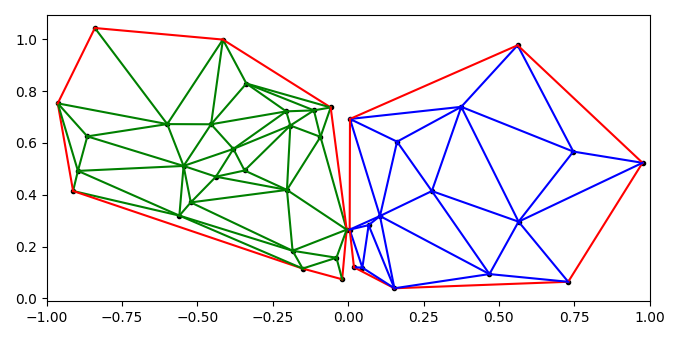
\includegraphics[width=0.70\textwidth]{Percussion2D.png}
    \caption{Disposition des floes de glace au moment de la percussion. Le floe de gauche (en vert) est muni d'une vitesse initiale non-nulle, alors que le floe de droite (en bleu) est au repos.}
    \label{fig:myfig}
  \end{figure}
\end{enumerate}


 
%----------------------------------------------------------------------------------------
%	ASSIGNMENT CONTENT - SECTION 2
%----------------------------------------------------------------------------------------

\section*{Difficultés rencontrées}


\begin{enumerate}
  \item La première est dans l'étude de la quantité de mouvement et de l'énergie totale du système 1D. Je reste convaincu que le problème est dû à la formule de calcul de l'énergie dissipée par les frottements visqueux. Je n'ai cependant pas réussi à trouver une formule plus appropriée (ni en ligne, ni par heuristique). S'il vous plait, j'aurais grand besoin d'aide là-dessus.
  \item La deuxième difficulté est liée à la percussion 2D. Remarquons que dans la simulation en pièce jointe, deux noeuds du floe de droite sont toujours fixes : \emph{c'est l'astuce qu'avait introduit Dimitri pour éviter des déplacements "aberrants"}. On observe le même problème sur le floe de gauche dans la vidéo (malgré la fixation de certains noeuds à droite seulement). \textbf{Es-ce vraiment un problème sachant que l'impulsion est presqu'instantannée} ? J'aurais besoin d'aide ici aussi, et je me demandais si vous seriez disponible cette semaine pour en discuter. 
  \item La troisième difficulté est moins urgente. En fait je n'ai pas implémenté de schéma symplectique pour les simulations 2D. Tout comme le code principal de Dimitri, j'ai juste utilisé les fonctions de \texttt{Scipy} implémentant ce schéma (elles sont plus rapide je crois). Mais je pense que ça serait un vrai plus d'apprendre comment fonctionnent ces schémas.
\end{enumerate}



%----------------------------------------------------------------------------------------
%	ASSIGNMENT CONTENT - SECTION 3
% ----------------------------------------------------------------------------------------
\section*{Travail à venir}

\emph{Par ordre de priorité :}


\begin{enumerate}
  \item Implémentation de l'interface web pour la percussion 2D suivant le modèle \texttt{Flask} de Dimitri, pour aider dans la validation du modèle.
  \item Étude du schéma symplectique, des valeurs propres, etc. et validation du modèle.
  \item Étude du code de \textbf{Matthias} et détermination de la durée de l'impulsion et des vitesses (d'ensemble) des floes après choc. 
  \item Même sans le code de Matthias, je pourrais peut-être commencer à étudier la fracturation \emph{pendant que les floes sont encore en contacts}.
\end{enumerate}



 
% %-------------------------------------------------------------------------------
% %							THE BIBLIOGRAPHY
% %-------------------------------------------------------------------------------
\clearpage   % Pour retirer les references de la bare de navigation
% \printbibliography


\end{document}
